\documentclass[10pt,twocolumn,letterpaper]{article}

\usepackage{cvpr}
\usepackage{times}
\usepackage{epsfig}
\usepackage{graphicx}
\usepackage{amsmath}
\usepackage{amssymb}
\usepackage{subfig}
\usepackage{float}

% Include other packages here, before hyperref.

% If you comment hyperref and then uncomment it, you should delete
% egpaper.aux before re-running latex.  (Or just hit 'q' on the first latex
% run, let it finish, and you should be clear).
\usepackage[breaklinks=true,bookmarks=false]{hyperref}

\cvprfinalcopy % *** Uncomment this line for the final submission

\def\cvprPaperID{****} % *** Enter the CVPR Paper ID here
\def\httilde{\mbox{\tt\raisebox{-.5ex}{\symbol{126}}}}

% Pages are numbered in submission mode, and unnumbered in camera-ready
%\ifcvprfinal\pagestyle{empty}\fi
\setcounter{page}{1}
\begin{document}

%%%%%%%%% TITLE
\title{Museum paintings retrieval and people detection}

\author{Marco Cagrandi\\
University of Modena and Reggio Emilia\\
Department of Engineering Enzo Ferrari\\
{\tt\small 203232@studenti.unimore.it}
% For a paper whose authors are all at the same institution,
% omit the following lines up until the closing ``}''.
% Additional authors and addresses can be added with ``\and'',
% just like the second author.
% To save space, use either the email address or home page, not both
\and
Alessio Ruggi\\
University of Modena and Reggio Emilia\\
Department of Engineering Enzo Ferrari\\
{\tt\small ??????@studenti.unimore.it}
\and
Daniele Lombardo\\
University of Modena and Reggio Emilia\\
Department of Engineering Enzo Ferrari\\
{\tt\small 202214@studenti.unimore.it}
}


\maketitle
%\thispagestyle{empty}

%%%%%%%%% ABSTRACT
\begin{abstract}
   Image processing, retrieval and people detection
   are important computer vision applications.
   Here we present our work on the ``Galleria Estense" dataset which contains
   videos and images from the ``Galleria Estense" of Modena.
   We propose a method to detect and retrieve the paintings, the statues and the people in the 
   museum based on different approaches: one with pure image processing and one 
   with YOLOv3 network, trained with a custom annotated dataset of paintings and statues 
   images. 
\end{abstract}

%%%%%%%%% BODY TEXT
\section{Introduction}

We have tackled the problem of detect paintings, statues and people in a museum (the Galleria Estense).
Our objectives were: rectify the paintings correcting the perspective distortions, retrieve the correct paintings in the dataset, provide a precise segmentation of both detected paintings and statues, sum up all the information we had and link the paintings and the people to a precise room in the museum.
 In order to achive our results, as further discussed in section 3, many techniques are involved: image processing topics as edge detection, connected components analysis, relevant ROI detection, object segmentation; image retrieval; deep learning and neural networks. 

\subsection{The dataset}

The dataset contains videos and images from the ``Galleria Estense" of Modena.

We have 208 short videos taken using different cameras, aspect ratios and resolutions. 
Some video was taken with a GoPro camera which introduced some distortion and
some video has frames particularly blurred due to the motion applied to the camera.

We have a database of 95 images that should represents all paintings of the ``Galleria Estense", 
but during the development of the project we realized that many paintings were missing 
and so we had to expand the paintings db adding some paintings taken from the ``Galleria Estense" 
website to improve the retrival and rectification tasks. We added 23 paintings that are named 
with a fixed suffix ``A" followed by a zero-based sequential identifier, \eg ``A000.jpeg".

Finally the dataset contains also a CSV file with informations for every painting present
in the db, including the position of the painting in the museum as a room number, and also an image
representing the plant of the museum to do the people detection task. When we expanded the 
painting db we expanded the CSV file accordingly to maintain consistency.

\section{Related works}

To detect the paintings and statues in the museum we trained a YOLOv3 network with
our custom annotated dataset. YOLO (acronym for ``You Only Look Once") is an object detection
network able to detect objects in images parsing the image only once, saving computation time w.r.t. 
other detection networks, however maintaining a good degree of precision.
We choosed YOLOv3 because it can achieve good performaces
both in terms of detection and speed as described in YOLOv3 paper:
\begin{quote}
   \cite{yolov3}
\end{quote}

\section{Approach}

The proposed approach involve several elements: Painting detection, Painting retrieval, 
Painting rectification, People detection and Statue detection.

\subsection{Painting Detection}

The first thing to do in order to detect relevant objects is to perform edge detection, but right before we have 
precessed the image with a gaussian filter in order to remove the gaussian noise and a bilateral filter. 
A good method to detect relevant edges is the Canny algorithm. It has been proposed with the following empirically determined thresholds 

\begin{table}[h!]
\begin{center}
\begin{tabular}{|l|c|}
\hline
\multicolumn{2}{|c|}{Thresholds}  \\
\hline
Low & High \\
\hline
400 & 400 \\ 
\hline
\end{tabular}
\caption{Canny thresholds}
\end{center}
\end{table}

with a Sobel operator with aperture of 5. With low threshold and high threshold set to an equal value, we don't accept weak edges, even if connected with strong edges.

The next step is to perform a Dilation 3x3 followed by an Erosion (Closing), in order to 
connect the edges of the same relevant object, and to detect the connected components in the output image 
thus obtaining a list of ROIs.
In order to discard unrelevant ROIs, we have set some rules that have to be satisfied in order to be considered
a relevant ROI: 
\begin{gather*}
	ratio_{ROI} =  \frac{max(width_{ROI}, height_{ROI})}{min(width_{ROI}, height_{ROI})} <  3 \quad (1)\\
	area_{ROI} > 0.015 \cdot area_{frame} \quad (2)\\ 
	max\_overlap = 0.8 \quad (3)
\end{gather*}

If the overlap is greater than the threshold, the bigger ROI survives.

We then propose an optional optimization, named \textbf{otsu\_optimization} and activated with the 
{\tt otsu\_opt\_enabled} flag set to True,
\begin{gather*}
	otsu\_th(ROI) > 1.3 \cdot otsu\_th(frame) \quad (4)
\end{gather*}
 where \(otsu\_th(x)\) is the function that computes the Otsu threshold. 
This optimization helps when it comes to discard the ROIs containing \eg wall sections,
but sometimes affects the paintings that are overexposed to the light.

\begin{figure}
    \centering
    \subfloat[Original frame]{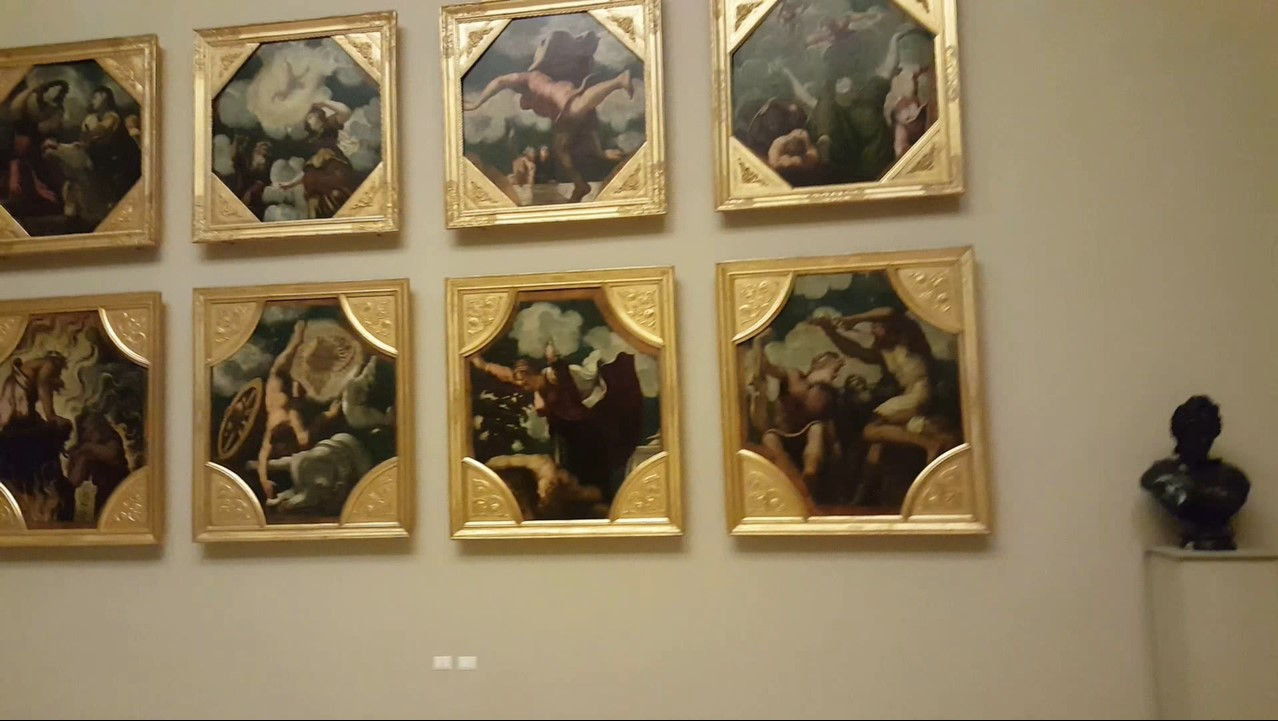
\includegraphics[width=0.5\linewidth]{frame.jpg}}\\
    \subfloat[Canny edge detection]{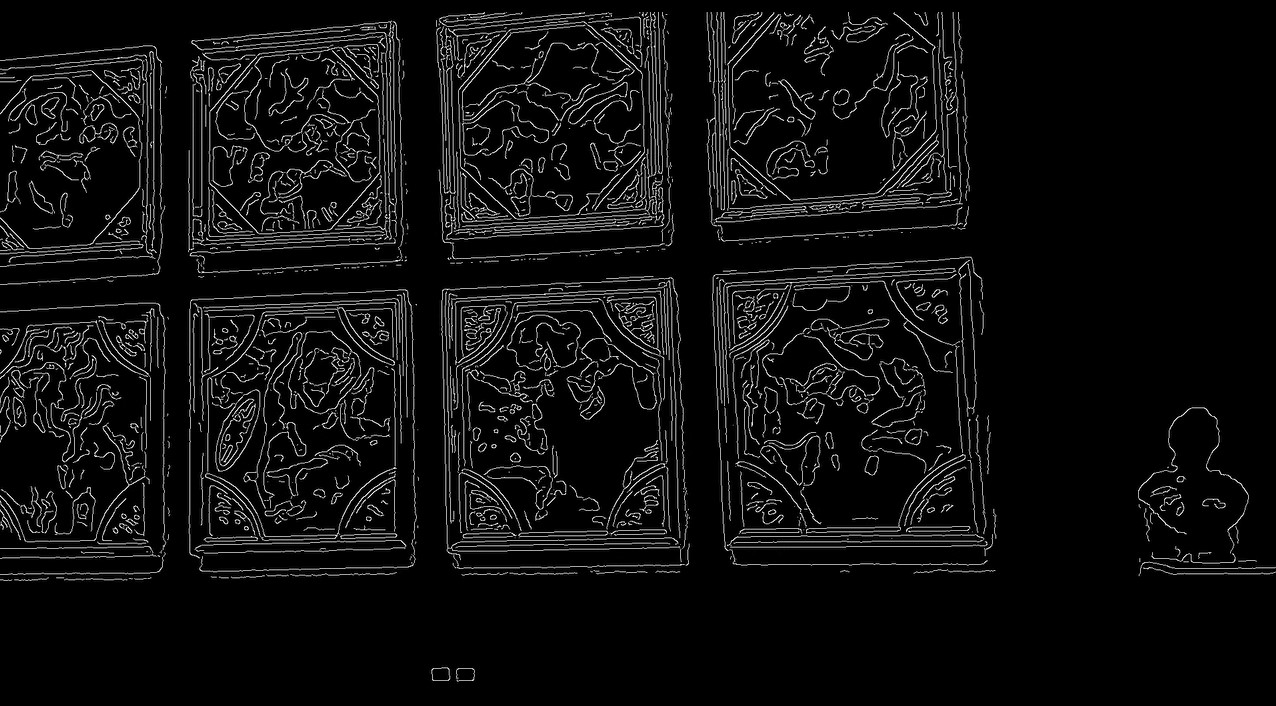
\includegraphics[width=0.5\linewidth]{canny_out.jpg}}\\
    \subfloat[Closing results]{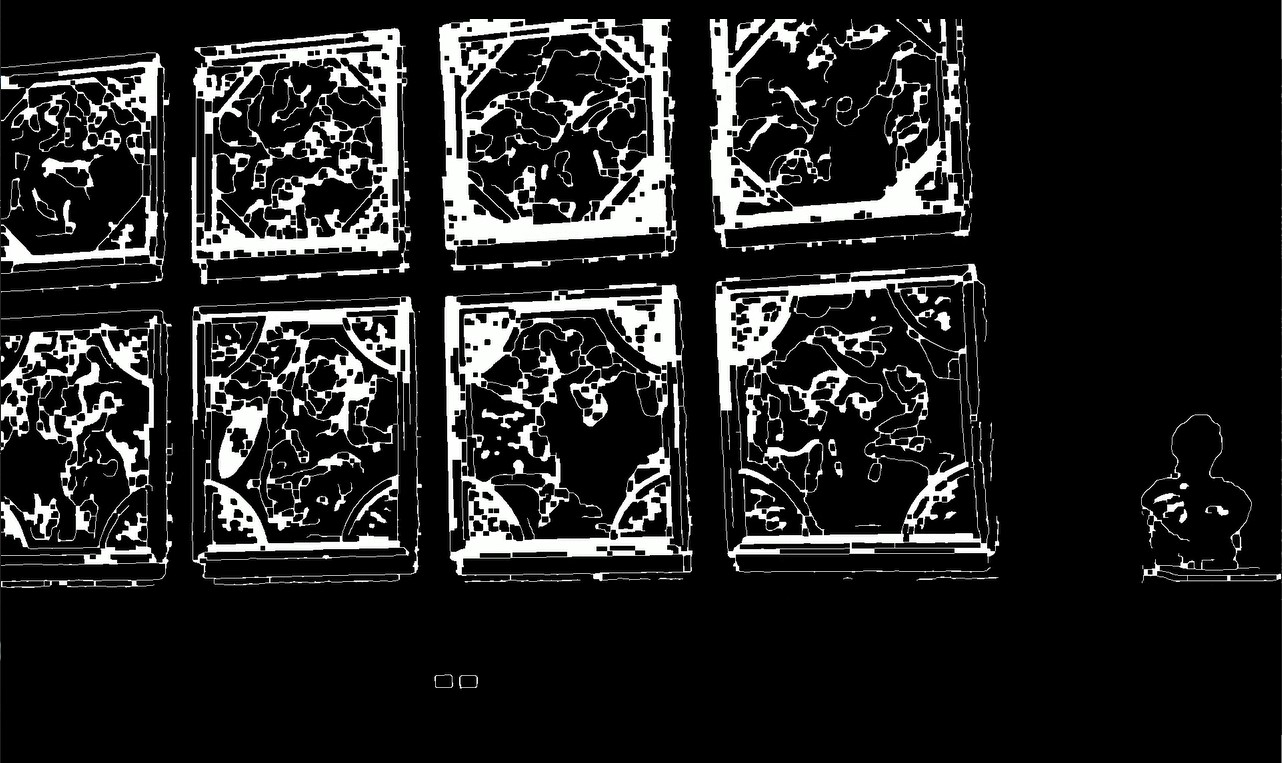
\includegraphics[width=0.5\linewidth]{closing_canny.jpg}}\\
    \subfloat[Detected connected components]{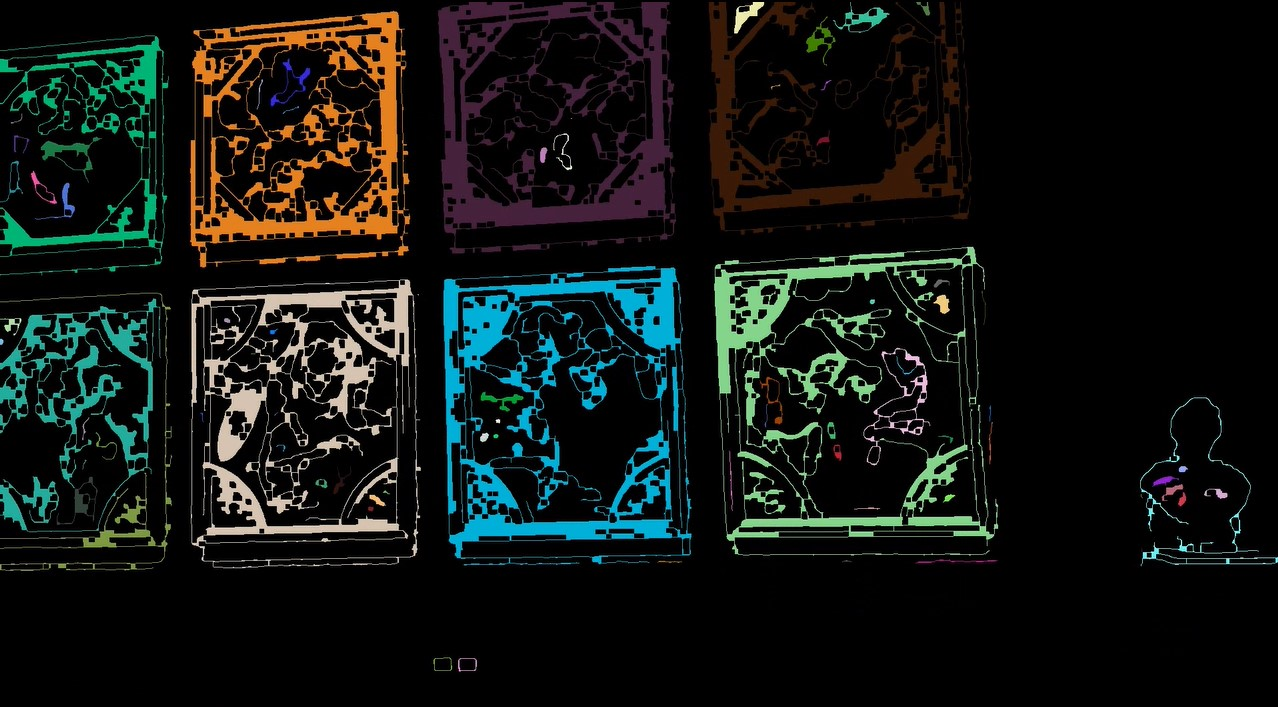
\includegraphics[width=0.5\linewidth]{connected_components.jpg}}\\
    \subfloat[Connected components ROIs]{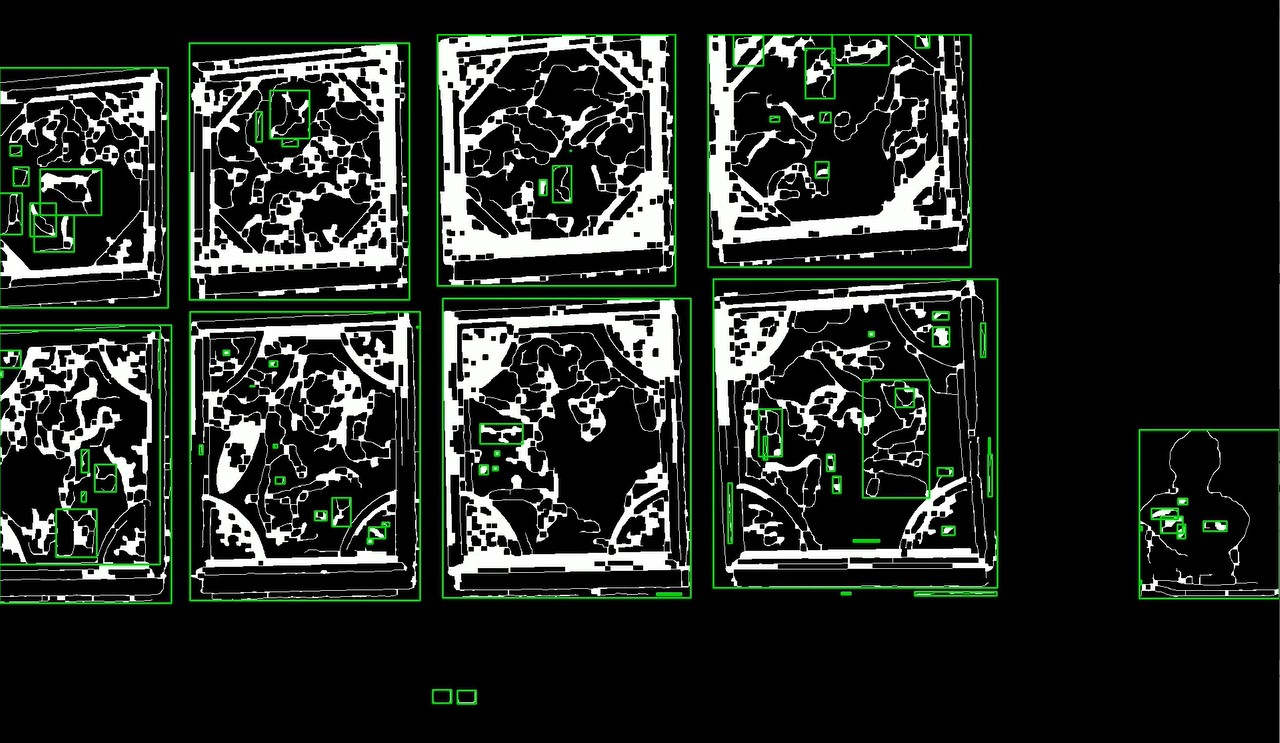
\includegraphics[width=0.5\linewidth]{components_rois.jpg}}\\
    \subfloat[Relevant ROIs; in green the discarded ROIs due to the overlap]{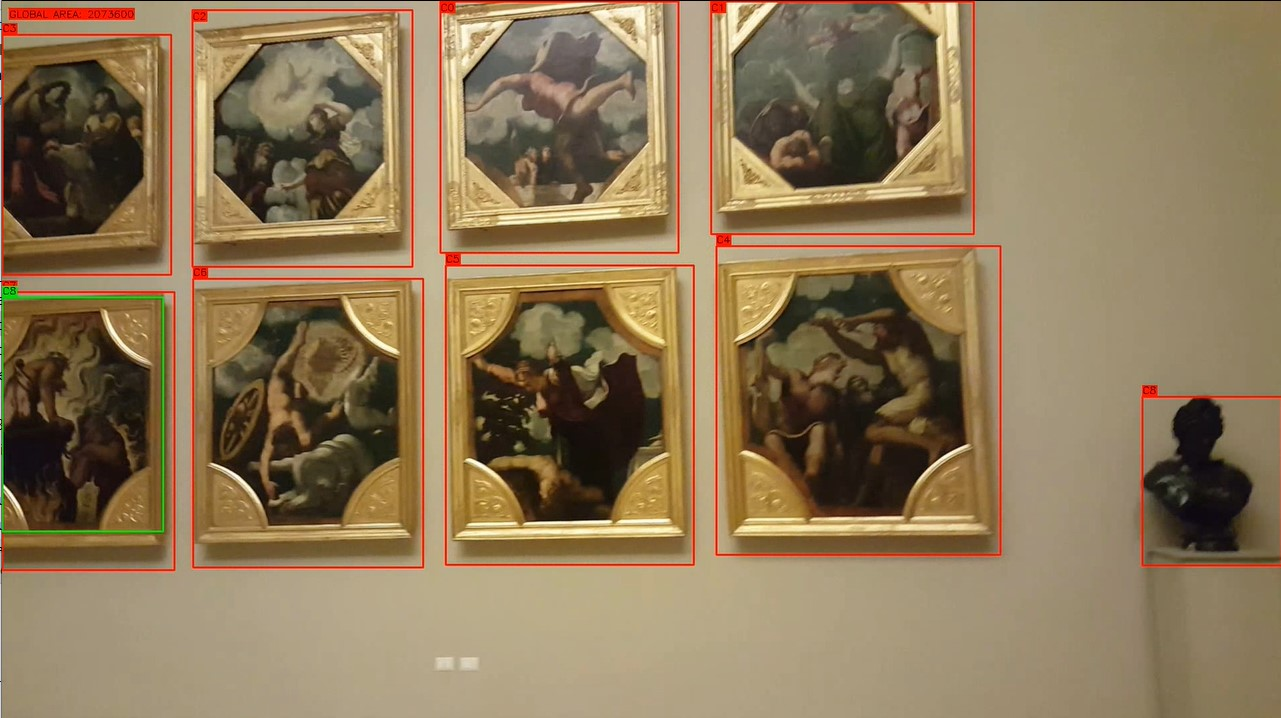
\includegraphics[width=0.5\linewidth]{relevant_rois.jpg}}
    \caption{Relevant ROIs results}
    \label{fig:foobar}
\end{figure}

\subsection{Painting Retrival}

\subsection{Painting Rectification}

\subsection{People Detection}

We used YOLOv3 network pre-trained on COCO dataset to detect people on videos, getting the returned
ROIs to draw them on output video.

\subsection{Statue Detection}

To detect the statues in the museum we fine-tuned the YOLOv3 network starting from
weights trained on COCO dataset. At the beginning we thought to detect statues and paintings
to improve the detection made with the Image Processing approach, so we trained the network
on 2 classes: Paintings and Statues.

We made our custom annotated dataset ripping frames from all videos of the museum, storing
them with a step of 250 frames for each video, obtaining 605 images mainly composed by paintings 
with only a 10\% of images containing statues.
We tried to train the network with this small and unbalanced dataset using different {\tt Learning Rate} 
values but the result was unsufficient.

After those tries we thought to use the network only to detect the statues, because the Image Processing
method was still better to detect paintings but often it wasn't able to detect statues.
So we learned the lesson and we tried to balance the dataset selecting manually frames with statues
from videos obtaining 282 images, each containg at least a statue with different point of views.
We annotated those images with more focus on statues than paintings, then we made a simple data 
augmentation script to flip all statues frames, obtaining 564 images with statues.
Finally our dataset contains 1169 images, slightly balanced in number of paintings and statues.

Using Adam optimizer with {\tt Non Maxima Suppression} value of 0.4, {\tt Confidence Threshold} of 0.8 
and a {\tt Learning Rate} of 0.004 we achieved an AP of {\bf 6.39\%}, considering also the painting class that we 
discarded in detection phase. 

To train the network we used an Nvidia GTX 1050 with 4Gb and it took us almost 4 days to
reach the 242th epoch with a batch size of 2, then we just stopped the training due to overfitting on 
{\tt confidence loss} [2]. 
We achieved the best results of AP with the 177th epoch and we used those weights to detect
statues on videos trying different combinations of {\tt Non Maxima Suppression} and {\tt Confidence Threshold} values,
defining them to 0.1 and 0.98 respectively.

\subsection{Segmentation}

\section{Results}

In this section, some results frame and training graphs will be shown.

\begin{figure*}[t]
\begin{center}
    \subfloat[No otsu\_optimization, bad]{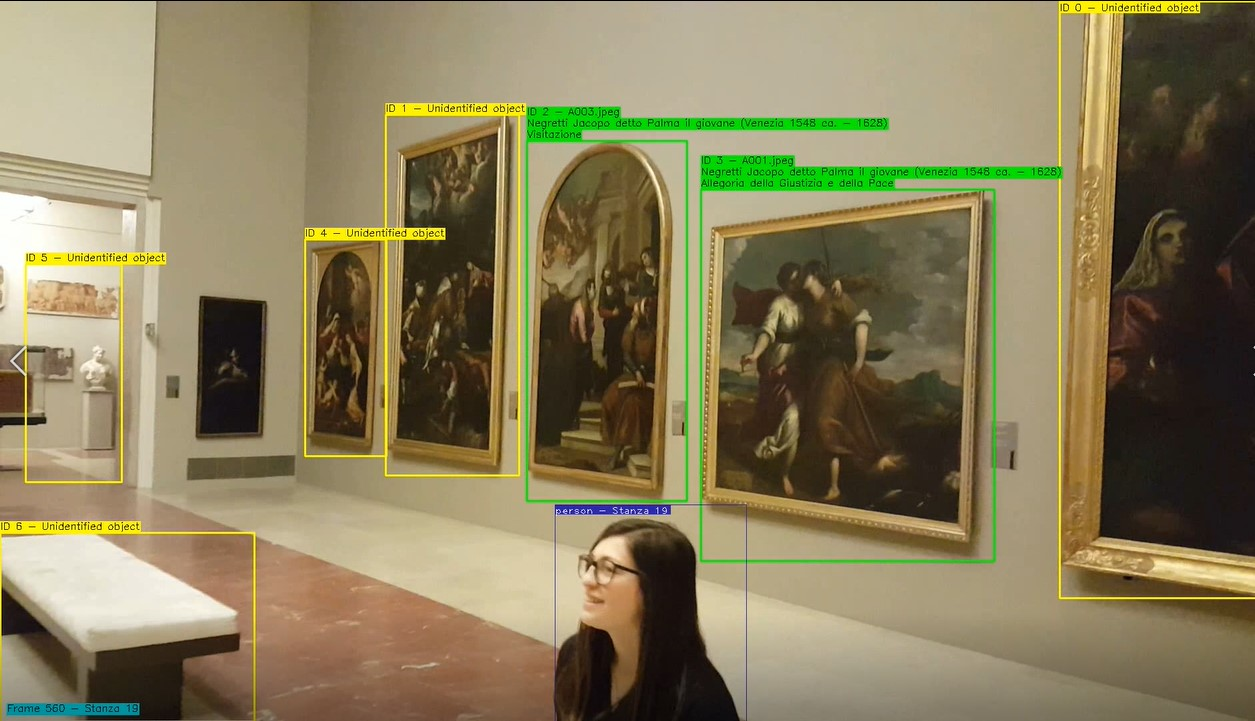
\includegraphics[width=0.5\linewidth]{4720_Frame560_noOtsu_bad.jpg}}
    \subfloat[With otsu\_optimization, good]{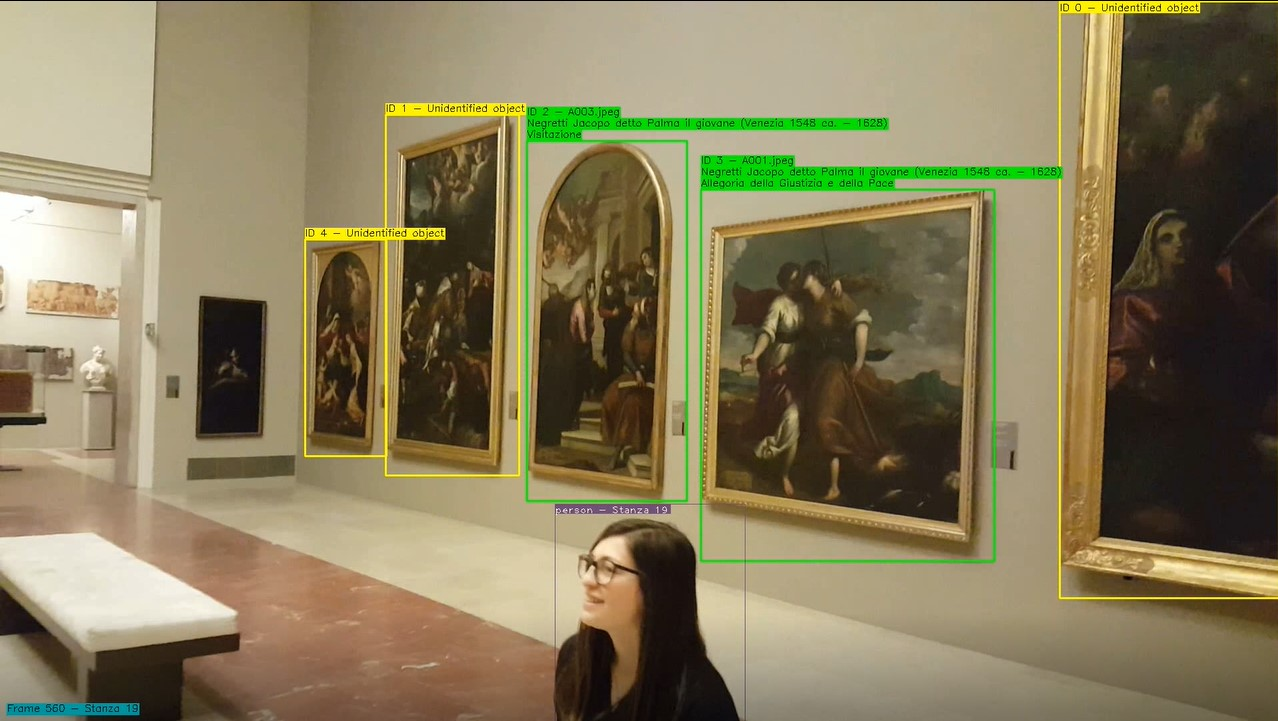
\includegraphics[width=0.5\linewidth]{4720_Frame560_yesOtsu_good.jpg}}\\
    \subfloat[No otsu\_optimization, good]{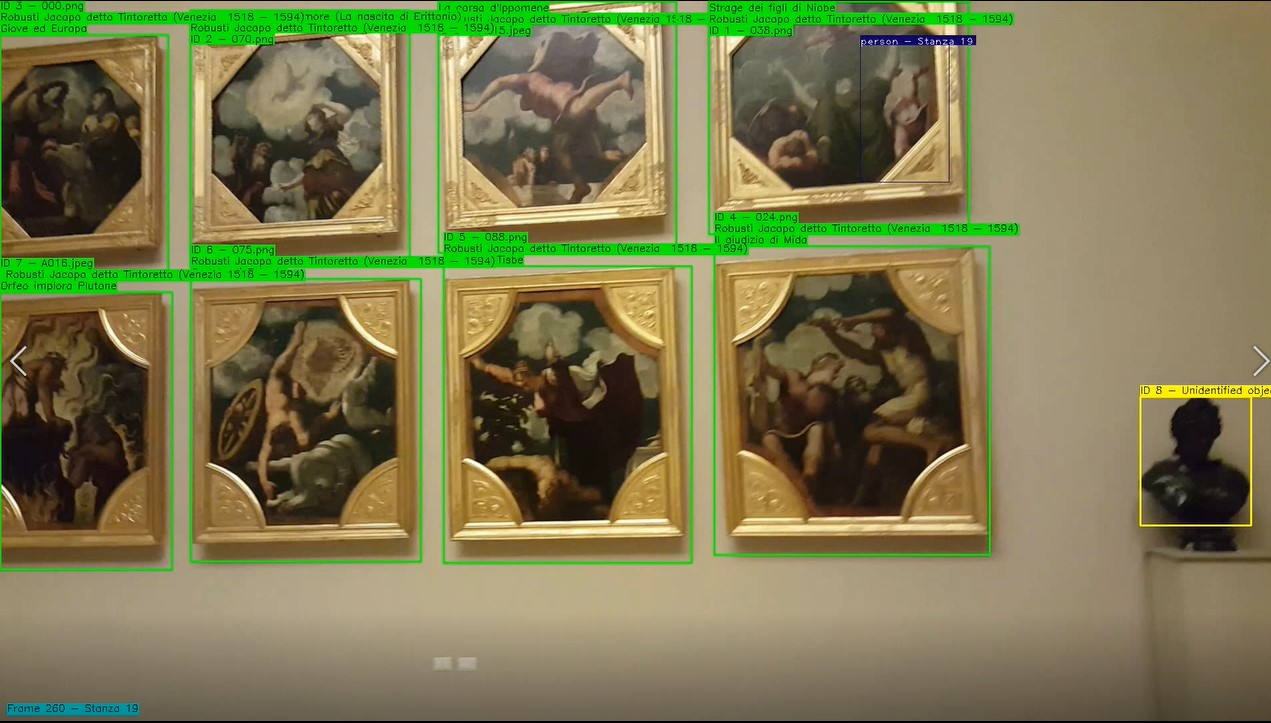
\includegraphics[width=0.5\linewidth]{4720_Frame260_noOtsu_Good.jpg}}
    \subfloat[With otsu\_optimization, bad]{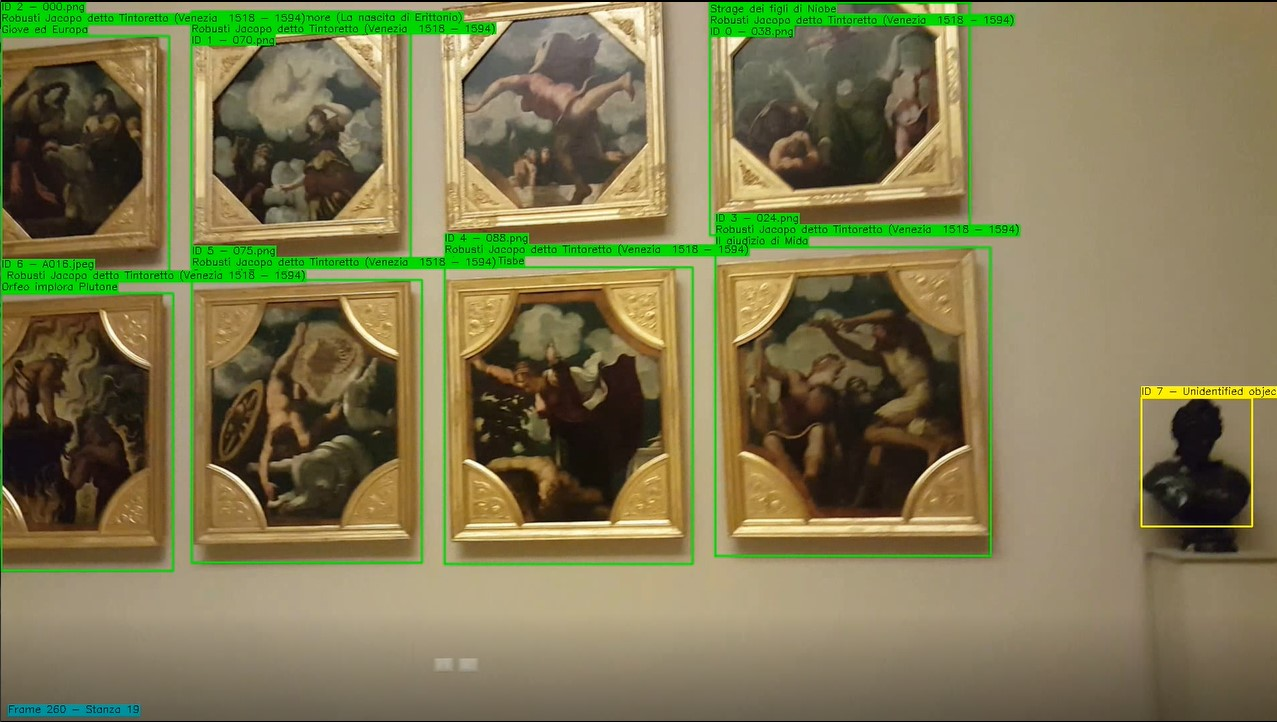
\includegraphics[width=0.5\linewidth]{4720_Frame260_yesOtsu_bad.jpg}}
\end{center}
   \caption{Example of otsu\_optimization (no statue detection nor segmentation)}
\label{fig:results1}
\end{figure*}

\begin{figure*}
    \centering
    \subfloat[]{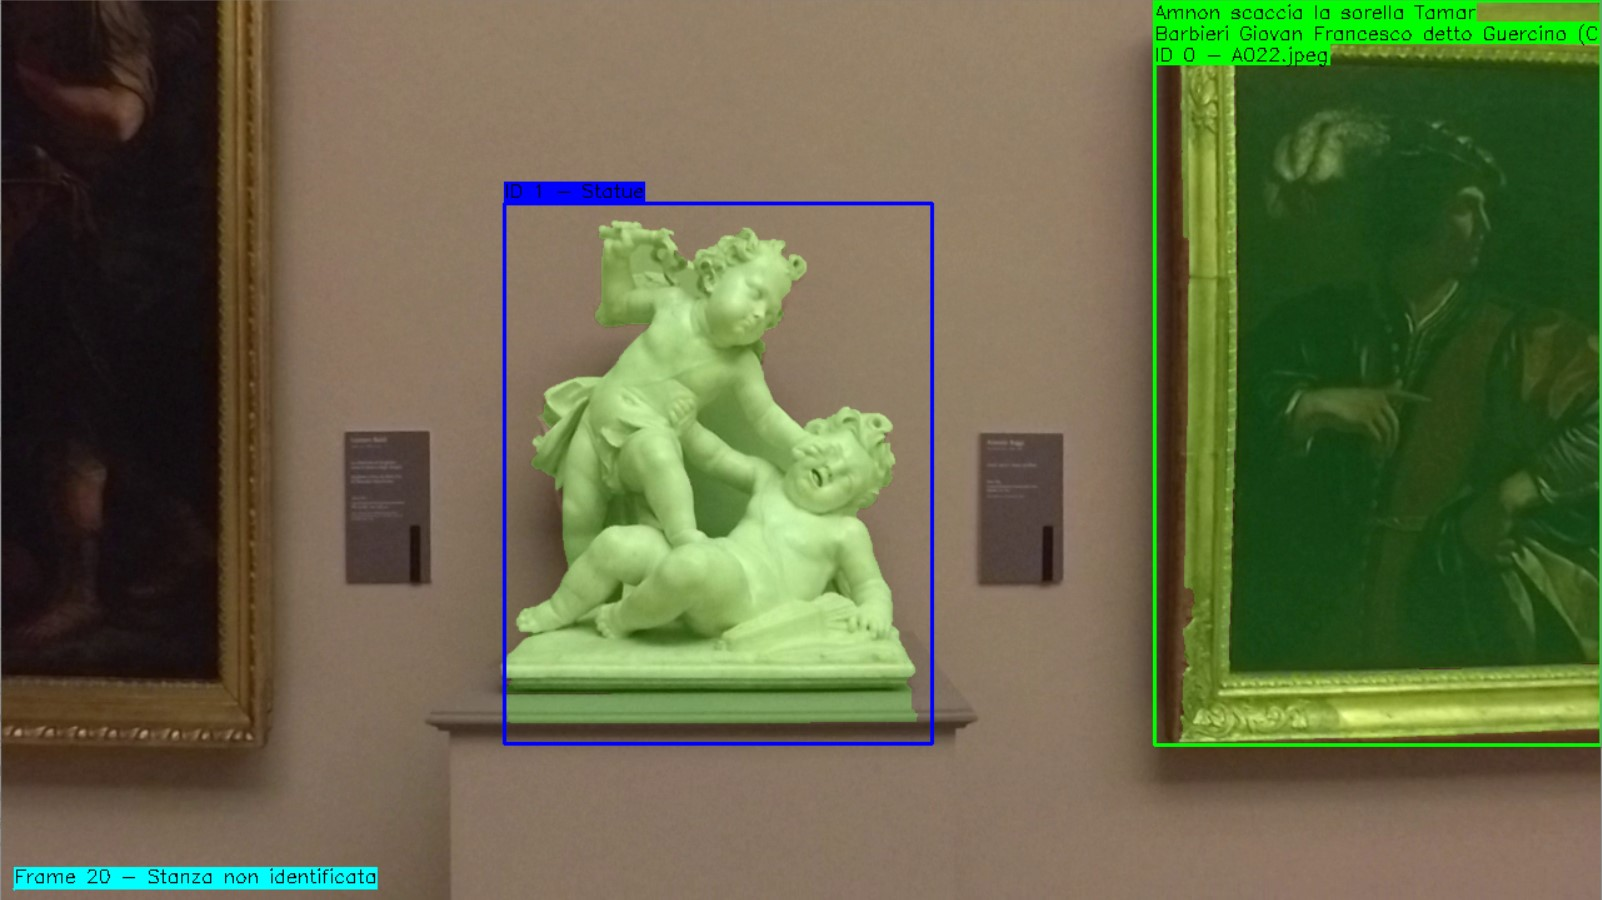
\includegraphics[width=0.5\linewidth]{good_segm_det_frame_20.jpg}}
    \caption{Example of segmentation and statue detection}
    \label{fig:foobar}
\end{figure*}

\begin{figure}
    \centering
    \subfloat[]{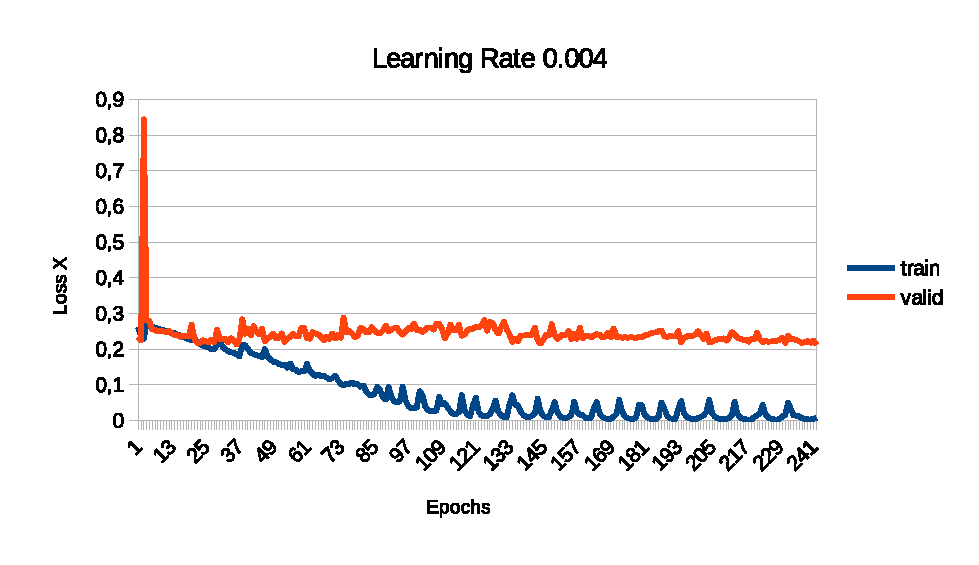
\includegraphics[width=0.5\linewidth]{loss_x.eps}}
    \subfloat[]{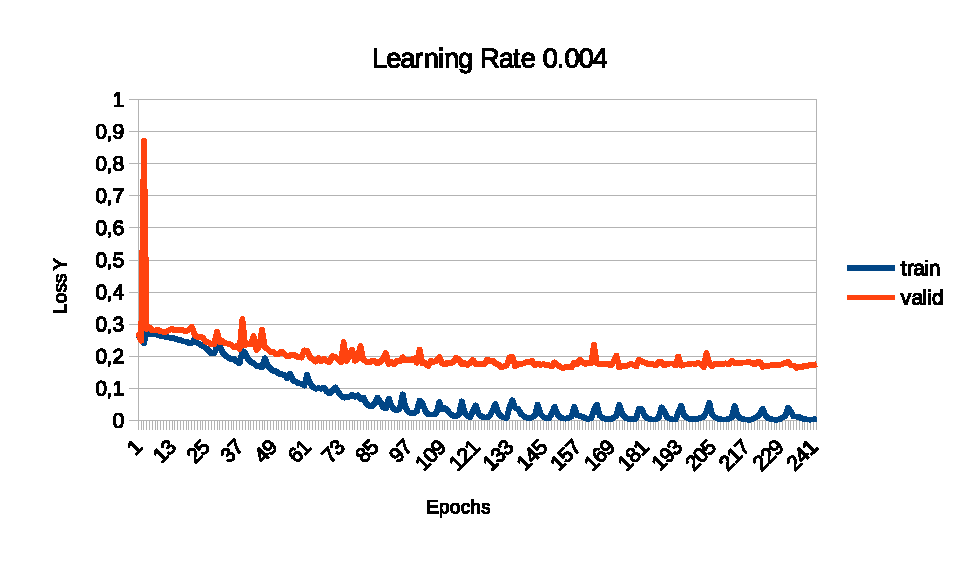
\includegraphics[width=0.5\linewidth]{loss_y.eps}}\\
    \subfloat[]{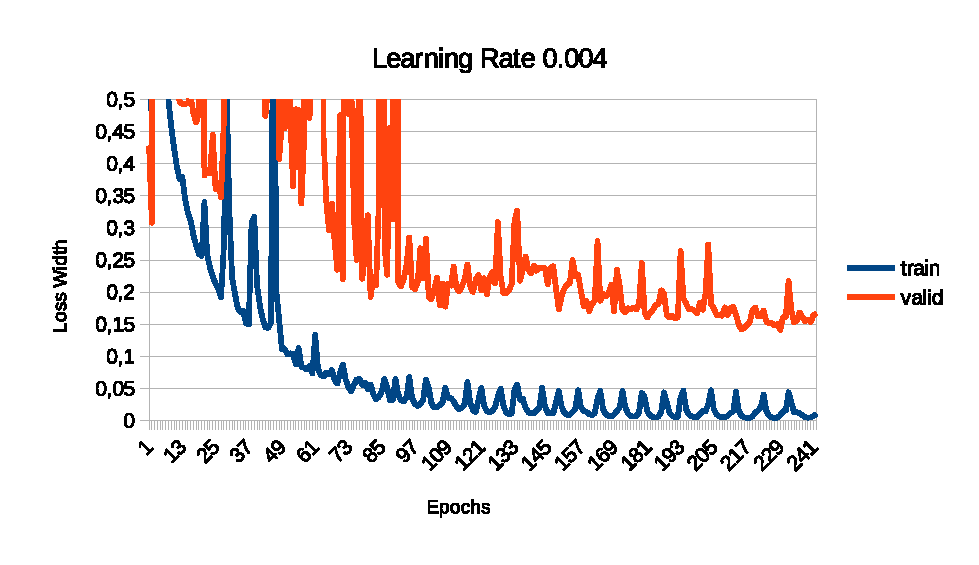
\includegraphics[width=0.5\linewidth]{loss_width.eps}}
    \subfloat[]{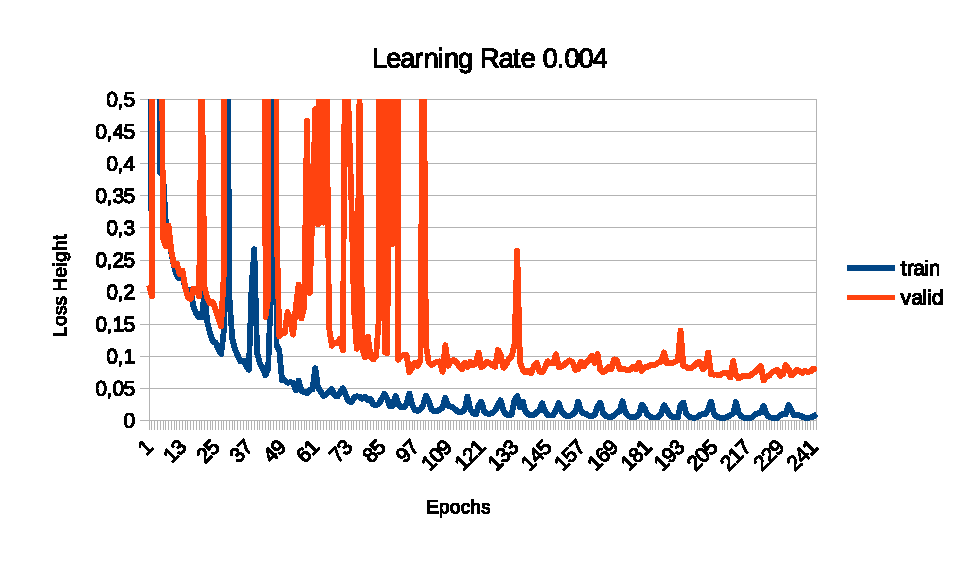
\includegraphics[width=0.5\linewidth]{loss_height.eps}}
    \caption{(a) Loss X, (b) Loss Y, (c) Loss Width and (d) Loss Height}
    \label{fig:foobar}
\end{figure}

\begin{figure}[t]
\begin{center}
   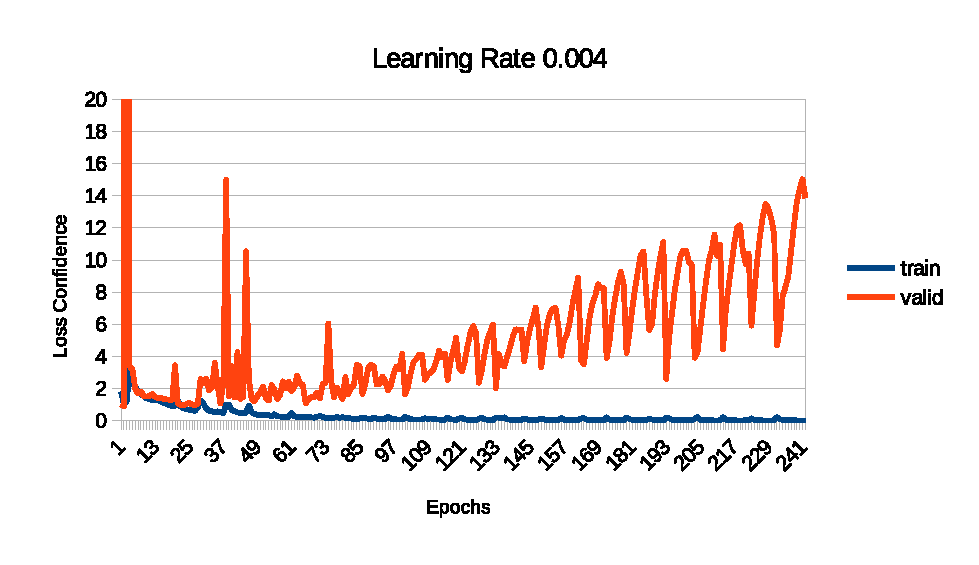
\includegraphics[width=1\linewidth]{loss_conf.eps}
\end{center}
   \caption{The Loss Confidence begins to overfit after few epochs, probably due to bad labeling of
paintings when we expanded the dataset.}
\label{fig:long}
\label{fig:onecol}
\end{figure}

\begin{figure}[t]
\begin{center}
   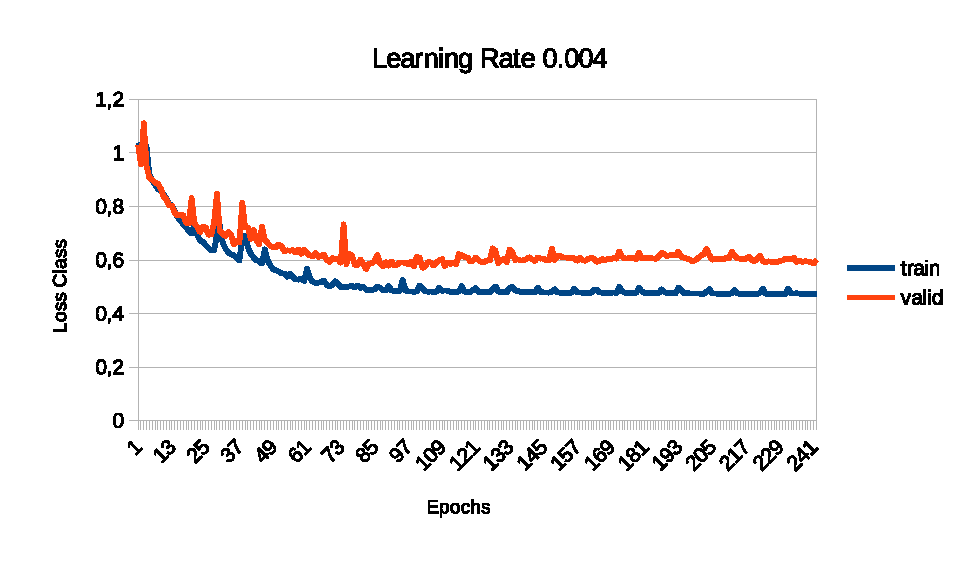
\includegraphics[width=1\linewidth]{loss_class.eps}
\end{center}
   \caption{The Loss Class has a good trend.}
\label{fig:long}
\label{fig:onecol}
\end{figure}

\begin{figure}[t]
\begin{center}
   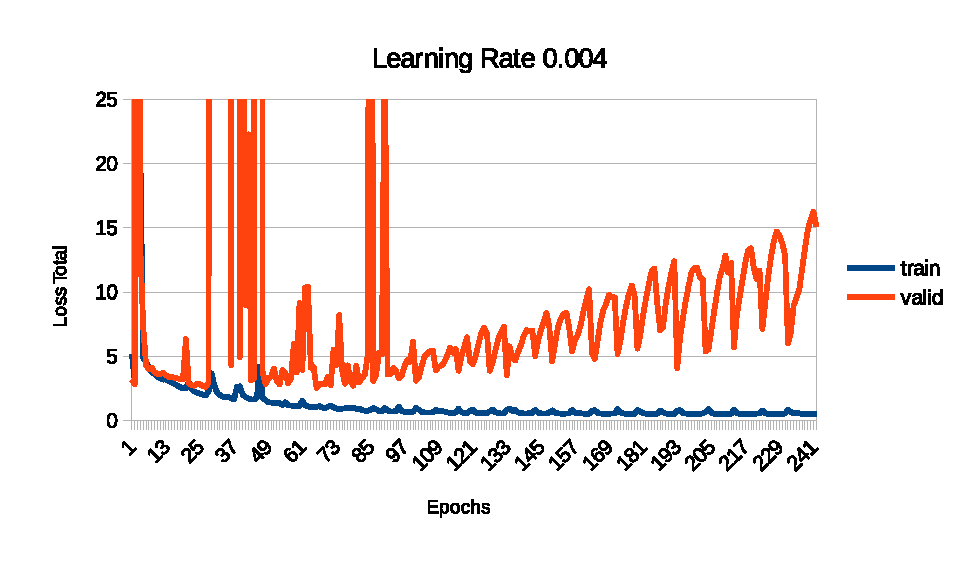
\includegraphics[width=1\linewidth]{loss_total.eps}
\end{center}
   \caption{The Total Loss is affected mainly by the loss confidence curve [2], 
while the loss class [3] and localization losses [1] are good enough to improve the precision [5].}
\label{fig:long}
\label{fig:onecol}
\end{figure}

\begin{figure}
    \centering
    \subfloat[]{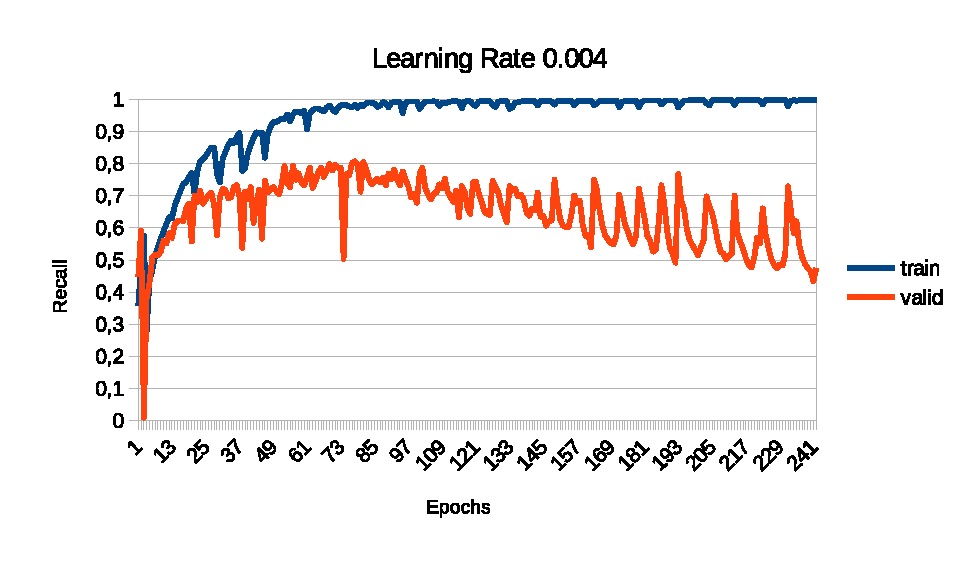
\includegraphics[width=0.5\linewidth]{recall.eps}}
    \subfloat[]{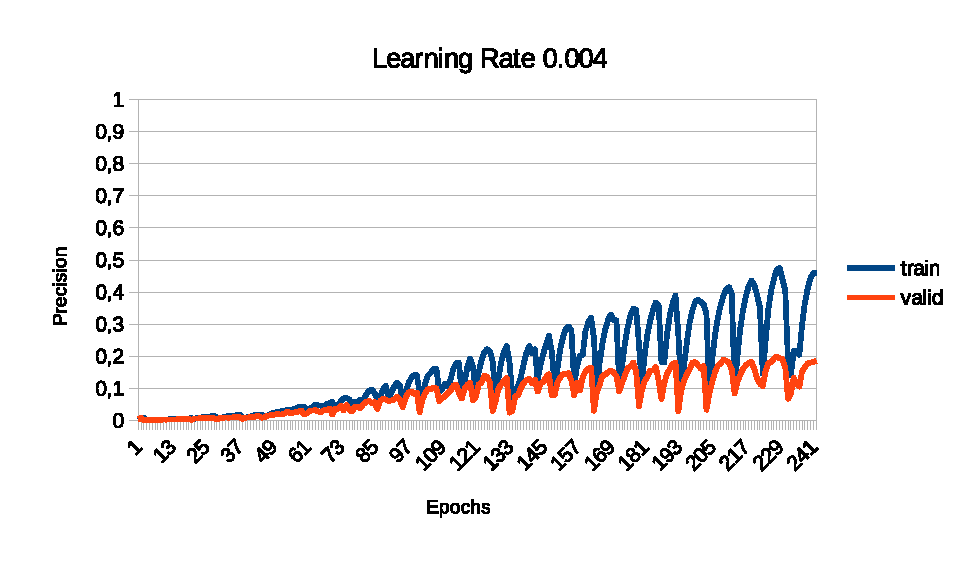
\includegraphics[width=0.5\linewidth]{precision.eps}}
    \caption{(a) Recall  and (b) Precision curves}
    \label{fig:foobar}
\end{figure}

\section{Discussion}

- migliorare la rete con dataset più ampio e bilanciato
- potremmo eliminare alcune ROI inutili (e.g. le etichette) utilizzando alcune tecniche di Image Processing
- Retrival, Rectification e Detection funzionerebbero meglio se avessimo un database di immagini completo anche con statue

%---------------------------------------------------------------------------------------------------------------------------------------------------------------------
% PER PRENDERE SPUNTO SUI DIVERSI COMANDI LATEX


\subsection{Language}

All manuscripts must be in English.

\subsection{Dual submission}

Please refer to the author guidelines on the CVPR 2019 web page for a
discussion of the policy on dual submissions.

\subsection{Paper length}
Papers, excluding the references section,
must be no longer than eight pages in length. The references section
will not be included in the page count, and there is no limit on the
length of the references section. For example, a paper of eight pages
with two pages of references would have a total length of 10 pages.
{\bf There will be no extra page charges for CVPR 2019.}

Overlength papers will simply not be reviewed.  This includes papers
where the margins and formatting are deemed to have been significantly
altered from those laid down by this style guide.  Note that this
\LaTeX\ guide already sets figure captions and references in a smaller font.
The reason such papers will not be reviewed is that there is no provision for
supervised revisions of manuscripts.  The reviewing process cannot determine
the suitability of the paper for presentation in eight pages if it is
reviewed in eleven.  

%-------------------------------------------------------------------------
\subsection{The ruler}
The \LaTeX\ style defines a printed ruler which should be present in the
version submitted for review.  The ruler is provided in order that
reviewers may comment on particular lines in the paper without
circumlocution.  If you are preparing a document using a non-\LaTeX\
document preparation system, please arrange for an equivalent ruler to
appear on the final output pages.  The presence or absence of the ruler
should not change the appearance of any other content on the page.  The
camera ready copy should not contain a ruler. (\LaTeX\ users may uncomment
the \verb'\cvprfinalcopy' command in the document preamble.)  Reviewers:
note that the ruler measurements do not align well with lines in the paper
--- this turns out to be very difficult to do well when the paper contains
many figures and equations, and, when done, looks ugly.  Just use fractional
references (e.g.\ this line is $095.5$), although in most cases one would
expect that the approximate location will be adequate.

\subsection{Mathematics}

Please number all of your sections and displayed equations.  It is
important for readers to be able to refer to any particular equation.  Just
because you didn't refer to it in the text doesn't mean some future reader
might not need to refer to it.  It is cumbersome to have to use
circumlocutions like ``the equation second from the top of page 3 column
1''.  (Note that the ruler will not be present in the final copy, so is not
an alternative to equation numbers).  All authors will benefit from reading
Mermin's description of how to write mathematics:
\url{http://www.pamitc.org/documents/mermin.pdf}.


\subsection{Blind review}

Many authors misunderstand the concept of anonymizing for blind
review.  Blind review does not mean that one must remove
citations to one's own work---in fact it is often impossible to
review a paper unless the previous citations are known and
available.

Blind review means that you do not use the words ``my'' or ``our''
when citing previous work.  That is all.  (But see below for
techreports.)

Saying ``this builds on the work of Lucy Smith [1]'' does not say
that you are Lucy Smith; it says that you are building on her
work.  If you are Smith and Jones, do not say ``as we show in
[7]'', say ``as Smith and Jones show in [7]'' and at the end of the
paper, include reference 7 as you would any other cited work.

An example of a bad paper just asking to be rejected:
\begin{quote}
\begin{center}
    An analysis of the frobnicatable foo filter.
\end{center}

   In this paper we present a performance analysis of our
   previous paper [1], and show it to be inferior to all
   previously known methods.  Why the previous paper was
   accepted without this analysis is beyond me.

   [1] Removed for blind review
\end{quote}


An example of an acceptable paper:

\begin{quote}
\begin{center}
     An analysis of the frobnicatable foo filter.
\end{center}

   In this paper we present a performance analysis of the
   paper of Smith \etal [1], and show it to be inferior to
   all previously known methods.  Why the previous paper
   was accepted without this analysis is beyond me.

   [1] Smith, L and Jones, C. ``The frobnicatable foo
   filter, a fundamental contribution to human knowledge''.
   Nature 381(12), 1-213.
\end{quote}

If you are making a submission to another conference at the same time,
which covers similar or overlapping material, you may need to refer to that
submission in order to explain the differences, just as you would if you
had previously published related work.  In such cases, include the
anonymized parallel submission~\cite{Authors14} as additional material and
cite it as
\begin{quote}
[1] Authors. ``The frobnicatable foo filter'', F\&G 2014 Submission ID 324,
Supplied as additional material {\tt fg324.pdf}.
\end{quote}

Finally, you may feel you need to tell the reader that more details can be
found elsewhere, and refer them to a technical report.  For conference
submissions, the paper must stand on its own, and not {\em require} the
reviewer to go to a techreport for further details.  Thus, you may say in
the body of the paper ``further details may be found
in~\cite{Authors14b}''.  Then submit the techreport as additional material.
Again, you may not assume the reviewers will read this material.

Sometimes your paper is about a problem which you tested using a tool which
is widely known to be restricted to a single institution.  For example,
let's say it's 1969, you have solved a key problem on the Apollo lander,
and you believe that the CVPR70 audience would like to hear about your
solution.  The work is a development of your celebrated 1968 paper entitled
``Zero-g frobnication: How being the only people in the world with access to
the Apollo lander source code makes us a wow at parties'', by Zeus \etal.

You can handle this paper like any other.  Don't write ``We show how to
improve our previous work [Anonymous, 1968].  This time we tested the
algorithm on a lunar lander [name of lander removed for blind review]''.
That would be silly, and would immediately identify the authors. Instead
write the following:
\begin{quotation}
\noindent
   We describe a system for zero-g frobnication.  This
   system is new because it handles the following cases:
   A, B.  Previous systems [Zeus et al. 1968] didn't
   handle case B properly.  Ours handles it by including
   a foo term in the bar integral.

   ...

   The proposed system was integrated with the Apollo
   lunar lander, and went all the way to the moon, don't
   you know.  It displayed the following behaviours
   which show how well we solved cases A and B: ...
\end{quotation}
As you can see, the above text follows standard scientific convention,
reads better than the first version, and does not explicitly name you as
the authors.  A reviewer might think it likely that the new paper was
written by Zeus \etal, but cannot make any decision based on that guess.
He or she would have to be sure that no other authors could have been
contracted to solve problem B.
\medskip

\noindent
FAQ\medskip\\
{\bf Q:} Are acknowledgements OK?\\
{\bf A:} No.  Leave them for the final copy.\medskip\\
{\bf Q:} How do I cite my results reported in open challenges?
{\bf A:} To conform with the double blind review policy, you can report results of other challenge participants together with your results in your paper. For your results, however, you should not identify yourself and should not mention your participation in the challenge. Instead present your results referring to the method proposed in your paper and draw conclusions based on the experimental comparison to other results.\medskip\\



\begin{figure}[t]
\begin{center}
\fbox{\rule{0pt}{2in} \rule{0.9\linewidth}{0pt}}
   %\includegraphics[width=0.8\linewidth]{egfigure.eps}
\end{center}
   \caption{Example of caption.  It is set in Roman so that mathematics
   (always set in Roman: $B \sin A = A \sin B$) may be included without an
   ugly clash.}
\label{fig:long}
\label{fig:onecol}
\end{figure}

\subsection{Miscellaneous}

\noindent
Compare the following:\\
\begin{tabular}{ll}
 \verb'$conf_a$' &  $conf_a$ \\
 \verb'$\mathit{conf}_a$' & $\mathit{conf}_a$
\end{tabular}\\
See The \TeX book, p165.

The space after \eg, meaning ``for example'', should not be a
sentence-ending space. So \eg is correct, {\em e.g.} is not.  The provided
\verb'\eg' macro takes care of this.

When citing a multi-author paper, you may save space by using ``et alia'',
shortened to ``\etal'' (not ``{\em et.\ al.}'' as ``{\em et}'' is a complete word.)
However, use it only when there are three or more authors.  Thus, the
following is correct: ``
   Frobnication has been trendy lately.
   It was introduced by Alpher~\cite{Alpher02}, and subsequently developed by
   Alpher and Fotheringham-Smythe~\cite{Alpher03}, and Alpher \etal~\cite{Alpher04}.''

This is incorrect: ``... subsequently developed by Alpher \etal~\cite{Alpher03} ...''
because reference~\cite{Alpher03} has just two authors.  If you use the
\verb'\etal' macro provided, then you need not worry about double periods
when used at the end of a sentence as in Alpher \etal.

For this citation style, keep multiple citations in numerical (not
chronological) order, so prefer \cite{Alpher03,Alpher02,Authors14} to
\cite{Alpher02,Alpher03,Authors14}.


\begin{figure*}
\begin{center}
\fbox{\rule{0pt}{2in} \rule{.9\linewidth}{0pt}}
\end{center}
   \caption{Example of a short caption, which should be centered.}
\label{fig:short}
\end{figure*}

%------------------------------------------------------------------------
\section{Formatting your paper}

All text must be in a two-column format. The total allowable width of the
text area is $6\frac78$ inches (17.5 cm) wide by $8\frac78$ inches (22.54
cm) high. Columns are to be $3\frac14$ inches (8.25 cm) wide, with a
$\frac{5}{16}$ inch (0.8 cm) space between them. The main title (on the
first page) should begin 1.0 inch (2.54 cm) from the top edge of the
page. The second and following pages should begin 1.0 inch (2.54 cm) from
the top edge. On all pages, the bottom margin should be 1-1/8 inches (2.86
cm) from the bottom edge of the page for $8.5 \times 11$-inch paper; for A4
paper, approximately 1-5/8 inches (4.13 cm) from the bottom edge of the
page.

%-------------------------------------------------------------------------
\subsection{Margins and page numbering}

All printed material, including text, illustrations, and charts, must be kept
within a print area 6-7/8 inches (17.5 cm) wide by 8-7/8 inches (22.54 cm)
high.
Page numbers should be in footer with page numbers, centered and .75
inches from the bottom of the page and make it start at the correct page
number rather than the 4321 in the example.  To do this fine the line (around
line 23)
\begin{verbatim}
%\ifcvprfinal\pagestyle{empty}\fi
\setcounter{page}{4321}
\end{verbatim}
where the number 4321 is your assigned starting page.

Make sure the first page is numbered by commenting out the first page being
empty on line 46
\begin{verbatim}
%\thispagestyle{empty}
\end{verbatim}


%-------------------------------------------------------------------------
\subsection{Type-style and fonts}

Wherever Times is specified, Times Roman may also be used. If neither is
available on your word processor, please use the font closest in
appearance to Times to which you have access.

MAIN TITLE. Center the title 1-3/8 inches (3.49 cm) from the top edge of
the first page. The title should be in Times 14-point, boldface type.
Capitalize the first letter of nouns, pronouns, verbs, adjectives, and
adverbs; do not capitalize articles, coordinate conjunctions, or
prepositions (unless the title begins with such a word). Leave two blank
lines after the title.

AUTHOR NAME(s) and AFFILIATION(s) are to be centered beneath the title
and printed in Times 12-point, non-boldface type. This information is to
be followed by two blank lines.

The ABSTRACT and MAIN TEXT are to be in a two-column format.

MAIN TEXT. Type main text in 10-point Times, single-spaced. Do NOT use
double-spacing. All paragraphs should be indented 1 pica (approx. 1/6
inch or 0.422 cm). Make sure your text is fully justified---that is,
flush left and flush right. Please do not place any additional blank
lines between paragraphs.

Figure and table captions should be 9-point Roman type as in
Figures~\ref{fig:onecol} and~\ref{fig:short}.  Short captions should be centred.

\noindent Callouts should be 9-point Helvetica, non-boldface type.
Initially capitalize only the first word of section titles and first-,
second-, and third-order headings.

FIRST-ORDER HEADINGS. (For example, {\large \bf 1. Introduction})
should be Times 12-point boldface, initially capitalized, flush left,
with one blank line before, and one blank line after.

SECOND-ORDER HEADINGS. (For example, { \bf 1.1. Database elements})
should be Times 11-point boldface, initially capitalized, flush left,
with one blank line before, and one after. If you require a third-order
heading (we discourage it), use 10-point Times, boldface, initially
capitalized, flush left, preceded by one blank line, followed by a period
and your text on the same line.

%-------------------------------------------------------------------------
\subsection{Footnotes}

Please use footnotes\footnote {This is what a footnote looks like.  It
often distracts the reader from the main flow of the argument.} sparingly.
Indeed, try to avoid footnotes altogether and include necessary peripheral
observations in
the text (within parentheses, if you prefer, as in this sentence).  If you
wish to use a footnote, place it at the bottom of the column on the page on
which it is referenced. Use Times 8-point type, single-spaced.


%-------------------------------------------------------------------------
\subsection{References}

List and number all bibliographical references in 9-point Times,
single-spaced, at the end of your paper. When referenced in the text,
enclose the citation number in square brackets, for
example~\cite{Authors14}.  Where appropriate, include the name(s) of
editors of referenced books.

\begin{table}
\begin{center}
\begin{tabular}{|l|c|}
\hline
Method & Frobnability \\
\hline\hline
Theirs & Frumpy \\
Yours & Frobbly \\
Ours & Makes one's heart Frob\\
\hline
\end{tabular}
\end{center}
\caption{Results.   Ours is better.}
\end{table}

%-------------------------------------------------------------------------
\subsection{Illustrations, graphs, and photographs}

All graphics should be centered.  Please ensure that any point you wish to
make is resolvable in a printed copy of the paper.  Resize fonts in figures
to match the font in the body text, and choose line widths which render
effectively in print.  Many readers (and reviewers), even of an electronic
copy, will choose to print your paper in order to read it.  You cannot
insist that they do otherwise, and therefore must not assume that they can
zoom in to see tiny details on a graphic.

When placing figures in \LaTeX, it's almost always best to use
\verb+\includegraphics+, and to specify the  figure width as a multiple of
the line width as in the example below
{\small\begin{verbatim}
   \usepackage[dvips]{graphicx} ...
   \includegraphics[width=0.8\linewidth]
                   {myfile.eps}
\end{verbatim}
}


%-------------------------------------------------------------------------
\subsection{Color}

Please refer to the author guidelines on the CVPR 2019 web page for a discussion
of the use of color in your document.

%------------------------------------------------------------------------
\section{Final copy}

You must include your signed IEEE copyright release form when you submit
your finished paper. We MUST have this form before your paper can be
published in the proceedings.

Please direct any questions to the production editor in charge of these
proceedings at the IEEE Computer Society Press: Phone (714) 821-8380, or
Fax (714) 761-1784.

{\small
\bibliographystyle{ieee_fullname}
\bibliography{egbib}
}

\end{document}
